\chapter{Evaluation}


% Things I need to evaluate.
% 
% Introduction about evaluation. The procedure and so on.
% 
% Generalisation evaluation.
% 
% Atomisation evaluation. 
% 
% Comparsion with the old procedure, i.e. the cummulative MI graph
% 
% Evaluation on an alternative dataset.
% 
% Evaluation of the full procedure:
% 
%  - comparison with the previous version
%     
%     - how accurate the pipeline is + how well does it extract concepts
%  
%  - comparison with a pipeline without concepts
% 
% 
% Conclusion which will include limitation

% TODO: move metric discussion here

In this chapter, we will discuss how well do the modifications made in this thesis perform. 
The evaluations can be divided into two categories, evaluations independent and within the context of the concept bottleneck pipeline.
The former helps us determine whether the implemented methods work sufficiently well, while the latter quantifies how much of an improvement have we made compared to the \ref{inherited-work}.

We will see the following evaluations independent of the concept bottleneck pipeline:
\begin{itemize}
    \item Performance of concept generalisation and its learning characteristics.
    \item Performance of atomisation and its learning characteristics.
    \item Joint performance of atomisation and generalisation.
    \item Applicability in a different domain.
\end{itemize}

The concept bottleneck pipeline dependent evaluation are compared with the previous work outlined in \ref{inherited-work}.
The following experiments are conducted:
\begin{itemize}
    % TODO: apparently informability is not a word.
    \item Evaluation of the new concept informability.
    \item Evaluation of the performance and explainability of the concept bottleneck pipeline with the new CoDEx module.
\end{itemize}
Finally, we will critically analyse the strengths and limitations of the implemented method and suggest areas for future improvement.

\section{Concept Bottleneck-Independent Evaluation}

\subsection{Metrics}

Both atomisation and generalisation problems had an set of solutions of unknown size.
As such, an ideal metric would higher score if 2 sets are very similar compared to those that are far apart.

That would ideally involve a similarity in number of produced solutions and similarity of the elements themselves.

Due to this reason, a single number would have been hard to interpret since it would make it unclear what kinds of mistakes the model is making. 
For that reason, the evaluation is done with metrics which work with sets with possibly reduced notion of element equality.

The simplest metrics used were per-example Jaccard Index, precision and recall, with exact equality.
Jaccard Index is a metric with the following form:

 - $Jaccard(A, B) = \frac{card(A \cap B)}{card(A \cup B)}$ where $card$ represents set cardinatlity, $A$ a set containing true solutions, while $B$ contains predicated solutions.\\
 
Precision and recall are equivalent to the following for the problems in this thesis:
 
  - $Precision(A, B) = \frac{number \; of \; correctly \; predicted \; sentences}{number \; of \; predicated \; sentences} = \frac{card(A \cap B)}{card(B)}$
  
  - $Recall(A, B) = \frac{number \; of \; correctly \; predicted \; sentences}{number \; of \; correct \; sentences} = \frac{card(A \cap B)}{card(A)}$ \\
where  $card$ represents set cardinatlity, $A$ a set containing true solutions, while $B$ contains predicated solutions.

These metrics are also evaluated in a slightly relaxed manner using Levensthein distance.
$Jaccard\text{-}k$ is a notation used in this report where two elements of a set are equal if their Levensthein distance is less or equal $k$.
The same notational trick is used for $Recall\text{-}k$ and $Precision\text{-}k$.

% TODO: rename precision and recall with generalisation-precision/generalistaion-recall


\subsection{Concept Generalisation}

\subsection{Concept Atomisation}

\subsubsection{Learning Characteristics}

The number of available examples was even smaller for atomisation, with only 94 examples available.
This task was more difficult to model and required a significantly larger search space with 17711 rules that could capture all of the rules hand-crafted solution relied on.
% INSERT ref to reducing the size of the search space
Note that this was the size of the search space even after the \#bias constraints eliminated rules which should not occur, using the procedure in X.
Being able to capture all hand-crafted rules is necessary so that the \textit{ILASP} can capture at least as good of a solution as the manually generated one.

% TODO: memory requirements of ILASP atomisation graph
As the task was much more complex to model, \textit{ILASP} also required much more memory to run as can be seen in X. 
Hence, the task was run on special machines with more RAM.
Alternatives reducing the search space that would avoid using a specialised machine, such as those with fewer possible body literals in a single rule, performed significantly worse than the hand-crafted solution.
As such, they are not considered further in this section.

% INSERT graph of learning run to completion.
Similar to the generalisation, an approximation of the best solution is returned after X iterations to decrease the running time of the system for a slightly worse solution.
In particular, a learning curve of the full run which influenced the decision can be seen in X.


\subsubsection{Results}
% INSERT this section when we have the data.

The results can be seen in the table below:

\begin{center}
\begin{tabular}{ |p{3cm}||p{3cm}|p{3cm}|p{3cm}|  }
 \hline
 \multicolumn{4}{|c|}{Summary of results} \\
 \hline
  &Accuracy&Precision&Recall\\ 
 \hline
 Training  & X $\pm$ Y & X $\pm$ Y & X $\pm$ Y \\
 Test & X $\pm$ Y & X $\pm$ Y & X $\pm$ Y \\
 \hline
\end{tabular}
\end{center}

Overall, the results are quite high with >90\% test average.
Looking into more detail the types of mistakes the model makes on the validation set, they can be subdivided into:

\begin{itemize}
    \item TODO
\end{itemize}


\section{Concept Bottleneck-Dependent Evaluation}

\subsection{Cumulative MI}

\subsubsection{Why does it matter?}

% INSERT ref MacKay book; maybe insert Venn diagram from Wikipedia.  
Mutual Information $I(X;Y)$ is defined as $I(X; Y) \equiv H(X) - H(X|Y)$. 
It estimates the average reduction in uncertainty about $x$ caused by understanding $y$'s value, or vice versa. 
It is the average quantity of information conveyed by $x$ regarding $y$.

In the context of this project, the discrete variable $Y$ is a set of label outcomes. A possible outcome is a number between 0 and 4 where each number represents an event which occurred.
The discrete variable $X$ represents a set of extracted concepts with size $k$, where $k$ is a parameter  tested in this evaluation.

In addition, given that the cumulative MI is under consideration, the set of size $k$ should ideally contain $k$ \emph{maximally informative} concepts, i.e. those which combined will result in a highest mutual information score.
% INSERT Luke and Vikranth's paper
However, finding such a set is infeasible as the problem is combinatiorial, but we can get a highly informative set by greedily adding a single concept that improves MI the most. 

So, by measuring cumulative MI we can find out how good the extracted concepts are at describing the labels.

\subsubsection{Results}

The results can be seen in \ref{cummulative-mi-graphs}.
It clearly shows that new concept extraction method greatly outperforms the old method.

\begin{figure}[h]
\caption{Cumulative MI graphs using old and new concept extraction pipeline}
\centering
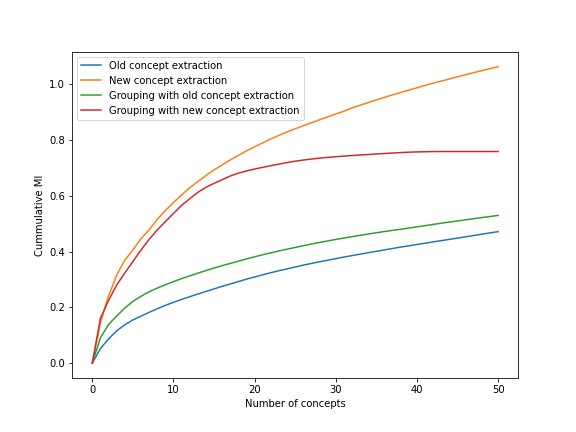
\includegraphics[width=\textwidth]{evaluation/Cummulative MI graphs.png}
\label{cummulative-mi-graphs}
\end{figure}


\subsection{Concept Bottleneck Pipeline Results}

In this subsection, we will see how does the new concept extraction perform when applied to the concept bottleneck pipeline.
The following models are compared in terms of explainability:
\begin{itemize}
    \item Concept Bottleneck Pipeline with old concepts.
    \item Concept Bottleneck Pipeline with new concepts.
\end{itemize}
In addition, two additional models are considered in performance measurements:
\begin{itemize}
    \item End-to-End model.
    \item MLB-Youtube model. 
\end{itemize}

% INSERT picture comparing architectures.
All three models intentionally have very similar architectures shown in X.
% INSERT hyper-parameter values
Moreover, the hyper-parameters are kept fixed at X across the runs for all models where we were in control of them


\subsubsection{Explainability}

% INSERT reference Mechanical Turk + original paper
As a part of \ref{inherited-work}, a Mechanical Turk study was preformed where the participants preferred the concept bottleneck results with attention in more than two-thirds of the cases.
Alternative choices were concept bottleneck results without attention, concepts of a random video from a different predicted class and a few randomly selected concepts from the set of most frequent concepts.


%  TODO: discuss with Luke and Ale about experiments
For this project a similar experiment was created. 
It additionally included a predicted set of concepts constructed with a new methods both before and after attention.

\subsubsection{Performance}


\subsection{Old Evaluation Stuff}

Despite this project being closely tied to the concept extraction from text, it will be researched and evaluated in the context of video classification.
Utilising human-based explanations to improve the video classification outcome is quite a novel area since there are no projects that do precisely so.
As such, there is no previous work the project will strive to do better than.\\

However, for the approach proposed in the project to be considered a success, it must:

 - Extract syntactic concept generalisations and create atomic sentences well. Both parts tasks will attempt to construct the solutions using machine learning/logic-based learning methods in a supervised setting. So, the methods proposed in this project should achieve small errors on relevant metrics.
 

 - Do better than previous work which the supervisors have completed. As mentioned in the section \ref{completed-work}, this project continues on the paper currently under review for the ICLR 2022 conference. So, improving upon the method presented in the referenced work is imperative.
 
 % INSERT reference
 - Outperform all attempts made on the MLB-YouTube \cite{RefWorks:RefID:3-piergiovanni2018fine-grained} dataset. The dataset used, MLB-V2E \cite{RefWorks:RefID:16-2021automatic}, has taken its video clips from the segmented MLB-YouTube dataset and augmented it with crowd-sourced explanations. Given that the explanations were created by candidates familiar with baseball rules, they should contain all information needed to make correct classifications. 
 In addition, Piergiovanni et al. \cite{RefWorks:RefID:3-piergiovanni2018fine-grained} argued that the MLB-YouTube is a challenging dataset to classify since the clips look similar. They are taken from the same camera angle, and the videos in different classes only differ by a fine-grained action.
 So, with explanations, the overall task is much easier.
 
 - Generalise to other datasets. The relevant metrics measuring error on concept generalisation and atomic sentence extraction should be similar when the method is applied to other datasets. It is possible to evaluate this project on the MSR-V2E \cite{RefWorks:RefID:16-2021automatic} dataset, which contains clips from everyday life and compare the performance with the MLB-V2E \cite{RefWorks:RefID:16-2021automatic} dataset.
 
 - Be scalable. The performance of the concept extraction pipeline should not deteriorate when a bigger number of examples is given. To evaluate the scalability requirement, multiple models will be trained with a different number of examples and their performances compared.
 
 - Be fast enough. This is a practical requirement. The machine learning model must not take too long to learn the needed representation. For example, it is unfeasible to have the model learn the concepts for more than 50 hours on the MLB-V2E dataset since one would need to evaluate it multiple times to facilitate the evaluation section of this project. Additionally, using the trained model on a test set example should be quick. The requirement mentioned will be measured by tracking how much time a model takes to complete a task.
 
 - Enable adding MLB-V2E explanations for a video quickly. The concepts constructed by this project will be grammatically correct sentences. So, given that a concept can be detected in the video, it should be easy to create multiple sentences out of it. Further evaluation plans within this area will be considered later, depending on the time available for video explanation generation. Possibilities include having subjects judge whether the explanation is: incorrect both grammatically and logically, incorrect only grammatically, incorrect logically, good.\\
 
The dataset with explanations is more costly and time-consuming to construct than the dataset without it.
So, the final evaluation should also quantify this requirement (e.g. in terms of volunteer hours spent) while judging the feasibility and success of classification with crowd-sourced explanations.